% !TEX root = ../document.tex

\chapter{\label{ch:tim}The Tim intermediate representation}

Before we discuss the Dynamix language, we must first take a detour and discuss the language that it targets. As briefly alluded to in \cref{ch:design}, Dynamix converts a language specification into a runnable program through the technique of \textit{meta-interpretation}\todo{better name} (see \cref{sec:design_evaluation}). However, instead of directly converting a source program into a sequence of Dynamix runtime instructions, we instead transform the source program into a more specialized \acf{IR} containing only the subset of Dynamix instructions that would actually be executed at runtime. By doing so, we can independently work on the Dynamix meta-language and the interpreter or compiler for the output \ac{IR}.\\

The specific \ac{IR} that Dynamix compiles\footnote{For the remainder of this thesis, whenever we use the term compilation within the context of Dynamix, it will refer to the process of meta-interpreting a Dynamix specification on a given input source. The name "compilation" is not inappropriate for this process. After all, Dynamix translates the input source to a lower-level specialized instruction set.} to is a new Spoofax meta-language called Tim\footnote{The name Tim originates from Target InterMediate language.}. Tim is a human-readable language with a relatively low level of abstraction that is designed to use \acf{CPS} (this choice coincides with the choice to use continuations as abstractions for control flow in Dynamix). Its grammar and semantics are largely inspired by the \ac{CPS} \ac{IR} used by the Standard ML compiler and described in Andrew W. Appel's book, Compiling with Continuations \cite{Appel1992}.\\

In this chapter, we discuss Tim's grammar (\cref{sec:tim_grammar}), dynamic semantics (\cref{sec:tim_runtime_semantics}), static semantics (\cref{sec:tim_static_semantics}), the Tim interpreter (\cref{sec:tim_interpreter}) and how it may be extended or improved upon in future work (\cref{sec:tim_future}).

\todo[inline]{perhaps a little introduction section to tim with examples here?}

\section{Design and grammar}
\label{sec:tim_grammar}
Tim as an intermediate representation centers around \acf{CPS} as a way of modeling control flow. As dicussed in chapter \ref{ch:design}, using a continuation-based approach to control flow modeling in a dynamic specification language is a natural way of allowing a wide-range of control flow while at the same time being able to take advantage of well-known compilation and optimization strategies available to \ac{CPS}-based languages.\\

Let us first discuss the grammar of Tim. Despite Tim being an \ac{IR} (and therefore not a language directly designed to be used by users), it has a properly defined syntax. This representation allows a user to inspect the output of a Dynamix compilation, write code directly in the target representation (which may be useful if Dynamix does not expose the necessary facilities to do so), and will also help us consider the semantics of Tim without needing to resort to abstract representations of terms. Note that this is unlike the \ac{CPS} \ac{IR} from "Compiling with Continuations" \cite{Appel1992} that Tim is based on, which only considers the algebraic signature of the IR and has no formal syntax definition. \Cref{gr:tim} shows the full grammar for the Tim \ac{IR}.\\

\newcommand{\prodname}[1]{{\scriptstyle <}\textit{#1}{\scriptstyle >}}

\begin{grammar}[The grammar of the Tim intermediate representation.][][gr:tim]
  \firstcase{\prodname{program}}{\prodname{exp}}{}\\

  \firstcase{\prodname{exp}}{\prodname{value}\textbt{(}\prodname{values}\textbt{)}}{Function tail call}
  \otherform{\textbt{\#}\prodname{primitive}\textbt{(}\prodname{values}\textbt{) => }\prodname{identifier}\textbt{; }\prodname{exp}}{Primitive call}
  \otherform{\textbt{\#}\prodname{primitive}\textbt{(}\prodname{values}\textbt{)}}{Primitive tail call}
  \otherform{\textbt{if \#}\prodname{primitive}\textbt{(}\prodname{values}\textbt{) then }\prodname{exp}\textbt{ else }\prodname{exp}}{Conditional primitive}
  \otherform{\textbt{fix \{ }\prodname{funs}\textbt{ \} in }\prodname{exp}}{Function definition}
  \otherform{\textbt{let }\prodname{bindings}\textbt{ in }\prodname{exp}}{Let definition}\\
  
  \firstcase{\prodname{value}}{\prodname{int literal}}{Integer literal}
  \otherform{\prodname{string literal}}{String literal}
  \otherform{\prodname{identifier}}{Variable reference}\\

  \firstcase{\prodname{values}}{\epsilon}{}
  \otherform{\prodname{value}}{}
  \otherform{\prodname{value}\textbt{, }\prodname{value}}{}\\

  \firstcase{\prodname{fun}}{\textbt{fun }\prodname{identifier}\textbt{(}\prodname{identifiers}\textbt{) = }\prodname{exp}}{}\\

  \firstcase{\prodname{funs}}{\epsilon}{}
  \otherform{\prodname{fun}}{}
  \otherform{\prodname{fun}\textbt{ }\prodname{funs}}{}\\

  \firstcase{\prodname{binding}}{\prodname{identifier}\textbt{ = }\prodname{value}}{}\\

  \firstcase{\prodname{bindings}}{\epsilon}{}
  \otherform{\prodname{binding}}{}
  \otherform{\prodname{binding}\textbt{, }\prodname{bindings}}{}\\

  \firstcase{\prodname{identifier}}{\texttt{[a-zA-Z\_\$] [a-zA-Z0-9\_\$-]*}}{}\\

  \firstcase{\prodname{identifiers}}{\epsilon}{}
  \otherform{\prodname{identifier}}{}
  \otherform{\prodname{identifier}\textbt{, }\prodname{identifiers}}{}\\

  \firstcase{\prodname{int literal}}{\texttt{'-'? [1-9] [0-9]*}}{}
  \firstcase{\prodname{string literal}}{\textbt{" }\prodname{string char}\textbt{* "}}{}
  \firstcase{\prodname{primitive}}{\texttt{[A-Za-z0-9\_+*/-]+}}{}
\end{grammar}

As you may note, Tim's grammar is very simple. At a first glance, one may think that this simplicity interferes with the design goals for Dynamix and Tim; after all, we desire for them to be generic enough to support a large variety of source languages. However, as we will discuss later (see also \cref{ch:case_studies}), just the small set of operations in Tim are enough to represent a wide range of source language paradigms.\\

Part of this expressiveness comes from the concept of primitive calls. Primitives are Tim's approach to compiler intrinsics: functions whose body is implemented directly by the Tim compiler or runtime. Through primitives, Tim can expose operations like integer addition and access to composite data structures without the need to introduce explicit new grammar for these actions. Tim also diverges from the \ac{IR} used in "Compiling with Continuations" in this aspect: while both \acp{IR} have the concept of primitive operations, the \ac{IR} used in Appel's book limits the available primitive operations to a fixed set, whereas primitives in Tim are allowed to be any valid identifier. Similarly, operations that have their own constructs in Appel's \ac{IR}, such as \texttt{RECORD} and \texttt{SWITCH}, are represented using primitive (tail) calls in Tim instead.\\

Primitives come in three forms: calls, tail calls, and conditionals. Primitive tail calls usually perform some form of control flow and as a result must appear in the tail call position. Non-tail calls to primitives do not break the \ac{CPS} expectation that calls must be in a tail call position: while primitives may look like function calls, their body is directly inlined and non-tail call primitives are not allowed to perform control flow. Conditional primitives\footnote{You may wonder why Tim has a separate if-then-else conditional primitive construct when such a construct can also be implemented by simply passing two separate continuations to a primitive tail call. The reason is simply because it allows Dynamix to have an if-then-else construct that directly correlates with a Tim construct. It has the added benefit of making Tim programs slightly more readable.} are only valid in if-then-else expressions and allow for conditional branching based on a compiler-implemented test (e.g. integer equality). An annotated example of a Tim program that uses primitives can be seen in \cref{fig:tim_example}. \\

One particular property of the Tim grammar, as well as its corresponding algebraic signature, is that it is \textit{\ac{CPS}-by-construction}. That is, the design of the grammar automatically enforces that certain properties of the \ac{CPS} hold for any well-formed Tim term. In particular, the grammar enforces that calls are always in the tail position, and that arguments to calls are atomic values (i.e. literals or variable references, but not complex sub-expressions).\\

\todo{tail call or tail call? green book uses both, wikipedia says tail call}
Enforcing proper tail call behavior is done by carefully modeling how multiple expressions combine. Instead of a sequencing operator (e.g. \texttt{exp ',' exp}) or a flat block statement (e.g. \texttt{'\{' exp* '\}'}), each expression in Tim directly embeds the next expression. The only expressions that do not specify their subsequent expression are function calls and primitive tail calls. This trivially makes them the final expression in a sequence, and hence enforces that every call is a tail call. Note that this property also means that every expression \textit{must} end in a tail call: it is simply not possible to terminate a sequence of expressions with anything other than a (primitive) tail call.\\

Enforcing that expressions (and function calls in particular) do not contain complex sub-expressions is done simply by making these a different sort. \textit{Values} are defined to be solely the expressions that directly yield a value: integer literals, string literals, and vriable references. Only values may be passed to function and primitive calls.\\

\begin{figure}
  \begin{tim}
// Functions within a fix block can refer to each other.
fix {
  fun main() =
    #print("Please input a number: ") => tmp0;

    // primitive tail call with two distinct continuations
    #read-number(onValidNumber, onInvalidNumber)
    
  fun onValidNumber(num) =
    // even simple arithmetic instructions are primitives
    #int-add(num, 1) => out;
    #print(out) => tmp0;
    #exit() // exit program
    
  fun onInvalidNumber() =
    #print("Invalid number entered.") => tmp0;
    main() // retry
} in
  main()
  \end{tim}
  \caption{A simple annotated Tim program that reads an integer value, increments it by one, and outputs it. If an invalid value is entered, an error message is displayed. Primitive calls are used to invoke I/O operations and arithmetic.}
  \label{fig:tim_example}
\end{figure}

\todo[inline]{or perhaps show some more tim examples here?}

\section{Dynamic semantics}
\label{sec:tim_runtime_semantics}
We will deviate a bit from the usual order in which languages are defined, and focus on the runtime semantics of Tim first. The reason why we will consider the runtime semantics first will become clear once we discuss the typing rules in \cref{sec:tim_operations}.\\

\subsection{Notation}
We formally define the runtime semantics of Tim through Kahn-style big-step operational semantics \cite{Kahn87:0}. To do so, let us first define some notation.\\

The store, $S$, is a mapping from variable names to their concrete value. Since Tim variables are immutable once created, we do not require a seperate environment and store. In order to still facilitate mutable values, we provide the heap, $H$, which functions as a mapping from address to value. The heap is not exposed to any Tim language constructs, but it may be freely accessed by the implementations of certain primitives. We use the syntax $S' = S[x \mapsto y]$ (respectively $H' = H[x \mapsto y]$) to extend $S$ with a new mapping from $x$ to $y$, yielding the store $S'$ (respectively heap $H'$). If $ S $ already contained a mapping for $ x $, it is \textit{shadowed} by the new value $ y $ in $ S' $, but remains accessible in $ S $. The syntax $S' = S[x/y]$ (respectively $H' = H[x/y]$) represents a store where the value bound to $ x $ is \textit{replaced} with $ y $. The syntax $ S[x] $ retrieves the value bound to $x$ in store $S$. \\

Runtime values are denoted as $v = X(a_1, a_2, ..., a_n)$. Here $X$ is the \textit{discriminant}, indicating the type of the value. The content of the data is included in the arguments $a_1$ through $a_n$. The core Tim language has three different runtime values: $int(i)$, $str(s)$ and $func(S, args, body)$. For the function runtime value, the associated $S$ indicates the environment that the function closes over. Primitives can return additional data types, prefixed with \texttt{\#}. These data values are opaque to core Tim constructs and can only be handled by primitives that support these data types.\\

Since Tim uses \acf{CPS}, we will define an expression term as yielding a continuation $ C $. Such a continuation may either be $ cont(S, e) $, indicating that execution should continue at expression $ e $ with store $ S $, or $ exit() $, indicating that execution should stop. As we will see later, we can define execution of a program as repeatedly evaluating continuations until we reach the $ exit() $ term.\\

We will use two different relations to define the behavior of Tim. For values\footnote{With values, we mean the "value" term type from the Tim grammar, indicating an atomic expression. When needed, we'll use the terms "value term" and "runtime value" to disambiguate between the two.}, we'll use the notation $ S, H \vdash e : v $ to indicate that the value term $ e $ evaluates to the runtime value $ v $ within the store $ S $ and heap $ H $. Since value terms cannot have side effects, we do not have to consider any changes to $ S $ or $ H $. For expressions, we use the notation $ S, H \vdash e \rightarrow C, H' $ to indicate that evaluating the expression $ e $ yields a continuation $ C $. We do not need to yield an $ S' $, as the continuation already contains the store to be used for subsequent expressions.

\subsection{Semantics of the core language}
With the notation defined, we can discuss the semantics of the Tim core\footnote{We define "Tim core" to be the parts of the Tim language that are statically defined, i.e. anything but the behavior of primitives.} language. Let us start simple by defining the behavior of values. String and integer literals directly convert to their runtime equivalents. For variables, we perform a lookup in the store.

\begin{prooftree}
  \AxiomC{}
  \RightLabel{\textsc{V-Int Literal}}
  \UnaryInfC{$S, H \vdash i : int(v)$}
\end{prooftree}

\begin{prooftree}
  \AxiomC{}
  \RightLabel{\textsc{V-String Literal}}
  \UnaryInfC{$S, H \vdash s : str(s)$}
\end{prooftree}

\begin{prooftree}
  \AxiomC{$v = S[x]$}
  \RightLabel{\textsc{V-Variable Reference}}
  \UnaryInfC{$S, H \vdash x : v$}
\end{prooftree}

With values out of the way, let us tackle the expressions. A \texttt{let}-binding simply extends the store with a new name for a value. Newly defined variables are only visible in the body, and not in subsequent bindings of the same let.\todo{make a comment here about how we could've also returned $cont(H_n, b)$, but we're reserving that syntax for actual continuations?}

\begin{prooftree}
  \AxiomC{$S, H \vdash e_1 : v_1$}
  \noLine
  \UnaryInfC{$S_1 = S[x_1 \mapsto v_1]$}
  \noLine
  \UnaryInfC{$S, H \vdash e_2 : v_2$}
  \noLine
  \UnaryInfC{$S_2 = S_1[x_2 \mapsto v_2]$}
  \noLine
  \UnaryInfC{\vdots}
  \noLine
  \UnaryInfC{$S, H \vdash e_n : v_n$}
  \noLine
  \UnaryInfC{$S_n = S_{n-1}[x_n \mapsto v_n]$}
  \noLine
  \UnaryInfC{$S_n, H \vdash b \rightarrow C, H'$}
  \RightLabel{\textsc{E-Let}}
  \UnaryInfC{$S, H \vdash \textbt{let } x_1 = e_1, x_2 = e_2, ..., x_n = e_n\textbt{ in } b \rightarrow C, H'$}
\end{prooftree}

\texttt{fix} expressions are used to declare functions. Functions declared within the same \texttt{fix} block are allowed to refer to each other, as well as any variables declared in a higher scope (they \textit{capture} their scope). \todo{better notation that does not require recursive usage of S'?}\todo{better notation that isn't so W I D E}

\begin{prooftree}
  \AxiomC{$f_1 = func(S', args_1, body_1)$}
  \noLine
  \UnaryInfC{$f_2 = func(S', args_2, body_2)$}
  \noLine
  \UnaryInfC{\vdots}
  \noLine
  \UnaryInfC{$f_n = func(S', args_n, body_n)$}
  \noLine
  \UnaryInfC{$S' = S[name_1 \mapsto f_1, name_2 \mapsto f_2, ..., name_n \mapsto f_n]$}
  \noLine
  \UnaryInfC{$S', H \vdash b \rightarrow C, H'$}
  \RightLabel{\textsc{E-Fix}}
  \UnaryInfC{$S, H \vdash \textbt{fix \{ } \textbt{fun } name_1 \textbt{(} args_1 \textbt{) = } body_1 \cdots \textbt{fun } name_n \textbt{(} args_n \textbt{) = } body_n \textbt{ \} in } b \rightarrow C, H'$}
\end{prooftree}

The (tail) call expression can be used to call functions. For a call to be valid, it must resolve to a value of type $ func $ with a matching number of arguments. We substitute the argument names into a new environment based on the captured environment from the function, then return a continuation value indicating that execution should continue at the body of the called function.

\begin{prooftree}
  \AxiomC{$S, H \vdash id : func(S_f, args, body)$}
  \noLine
  \UnaryInfC{$ S, H \vdash a_1 : v_1 $}
  \noLine
  \UnaryInfC{$ S, H \vdash a_2 : v_2 $}
  \noLine
  \UnaryInfC{\vdots}
  \noLine
  \UnaryInfC{$ S, H \vdash a_n : v_n $}
  \noLine
  \UnaryInfC{$S_f' = S_f[args_1 \mapsto v_1, args_2 \mapsto v_2, ..., args_n \mapsto v_n]$}
  \noLine
  \UnaryInfC{$C = cont(S_f', body)$}
  \RightLabel{\textsc{E-Tail Call}}
  \UnaryInfC{$S, H \vdash id \textbt{(} a_1, a_2, ..., a_n \textbt{)} \rightarrow C, H $}
\end{prooftree}

The primitive tail call is very similar, but we defer the next continuation as well as the resulting heap to the implementation of the primitive. It is an error to call a primitive that is not defined. We discuss the semantics of several primitives in \cref{subsec:tim_primitive_semantics}.

\begin{prooftree}
  \AxiomC{$ S, H \vdash a_1 : v_1 $}
  \noLine
  \UnaryInfC{$ S, H \vdash a_2 : v_2 $}
  \noLine
  \UnaryInfC{\vdots}
  \noLine
  \UnaryInfC{$ S, H \vdash a_n : v_n $}
  \noLine
  \UnaryInfC{$ C, H' = \textsc{TailPrimitive}(H, \textbt{\#}$id$, v_1, v_2, ..., v_n) $}
  \RightLabel{\textsc{E-Primitive Tail Call}}
  \UnaryInfC{$S, H \vdash \texttt{\#} id \textbt{(} a_1, a_2, ..., a_n \textbt{)} \rightarrow C, H' $}
\end{prooftree}

Non-tail calls to primitives are similar, but instead of returning a continuation return a value directly. Note that even non-tail call continuations are allowed to change the heap.

\begin{prooftree}
  \AxiomC{$ S, H \vdash a_1 : v_1 $}
  \noLine
  \UnaryInfC{$ S, H \vdash a_2 : v_2 $}
  \noLine
  \UnaryInfC{\vdots}
  \noLine
  \UnaryInfC{$ S, H \vdash a_n : v_n $}
  \noLine
  \UnaryInfC{$ v, H_1 = \textsc{Primitive}(H, \textbt{\#}$id$, v_1, v_2, ..., v_n) $}
  \noLine
  \UnaryInfC{$ S' = S[x \mapsto v]$}
  \noLine
  \UnaryInfC{$ S', H_1 \vdash e \rightarrow C, H_2 $}
  \RightLabel{\textsc{E-Primitive Call}}
  \UnaryInfC{$S, H \vdash \texttt{\#} id \textbt{(} a_1, a_2, ..., a_n \textbt{) => } x \textbt{; } e \rightarrow C, H_2 $}
\end{prooftree}

Finally, conditional primitives are simply invoke the primitive function and branch based on the result of this invocation. It should be noted that the $true$ and $false$ in the semantics here are simply indications on which branch should be taken, with no particular requirements on exactly how these values are represented.

\begin{prooftree}
  \AxiomC{$ S, H \vdash a_1 : v_1 $}
  \noLine
  \UnaryInfC{$ S, H \vdash a_2 : v_2 $}
  \noLine
  \UnaryInfC{\vdots}
  \noLine
  \UnaryInfC{$ S, H \vdash a_n : v_n $}
  \noLine
  \UnaryInfC{$ b, H_1 = \textsc{ConditionalPrimitive}(H, \textbt{\#}$id$, v_1, v_2, ..., v_n) $}
  \noLine
  \UnaryInfC{$ e =\left\{\def\arraystretch{1.2}\begin{tabular}{@{}l@{\quad}l@{}}
    $e_1$ & if $b$ is $true$ \\
    $e_2$ & if $b$ is $false$
  \end{tabular}\right.$ }
  \noLine
  \UnaryInfC{$ S, H_1 \vdash e \rightarrow C, H_2 $}
  \RightLabel{\textsc{E-Primitive Conditional}}
  \UnaryInfC{$S, H \vdash \textbt{if \#} id \textbt{(} a_1, a_2, ..., a_n \textbt{) then } e_1 \textbt{ else } e_2 \rightarrow C, H_2 $}
\end{prooftree}

\subsection{Executing continuations to completion}
Now that we know the semantics of individual expressions, let us consider how to execute a Tim program to completion. To execute some program $ p $ (which consists of a top-level expression), we simply iteratively apply the appropriate dynamic semantics rule to yield a continuation $ C $. If this continuation is $ cont(S', e') $, we re-apply the appropriate rule for $ e' $. We halt once we reach the $ exit() $ continuation. We use the notation $ S, H \vdash e \Rightarrow C $ to indicate this operation, using the double arrow to indicate that we repeatedly apply the relation.

\begin{prooftree}
  \AxiomC{$S, H \vdash e \rightarrow cont(S', e'), H' $}
  \noLine
  \UnaryInfC{$ S', H' \vdash e' \Rightarrow C $}
  \RightLabel{\textsc{E-Program Recurse}}
  \UnaryInfC{$S, H \vdash e \Rightarrow C $}
\end{prooftree}

\begin{prooftree}
  \AxiomC{$S, H \vdash e \rightarrow exit(), \_ $}
  \RightLabel{\textsc{E-Program Exit}}
  \UnaryInfC{$S, H \vdash e \Rightarrow exit() $}
\end{prooftree}

\todo[inline]{elaborate more here? give an example of these rules being applied?}

\subsection{Semantics of various primitives}
\label{subsec:tim_primitive_semantics}
Now let us discuss the semantics of some of the primitives available to Tim programs. Since Tim offers an \acs{API} for language designers to implement their own primitives, it is impossible to provide an exhaustive list of all primitives and their semantics. Rather, this section is intended as a way to show how primitives may be implemented and how they are capable of significantly extending the features available to Tim programs. Appendix ??\todo{does it?} contains a full list of the semantics for primitives used in the case studies discussed in \cref{ch:case_studies}.\\

\noindent The \texttt{\#exit} primitive is the only way to gracefully terminate execution:

\begin{prooftree}
  \AxiomC{}
  \RightLabel{\textsc{Prim-Exit}}
  \UnaryInfC{$\textsc{TailPrimitive}(H, \textbt{\#exit}) = exit(), H$}
\end{prooftree}

\smallskip

\noindent Simple operations, such as integer addition, \texttt{\#int-add}, are expressed through primitives. But primitives are not limited to only performing a single operation: the \texttt{\#str-add} primitive performs string concatenation, a considerably more complex operation\footnote{An alternative approach would be to expose primitives to convert strings to and from character arrays, and having the user perform the concatenation of the two arrays themselves.}.

\begin{prooftree}
  \AxiomC{}
  \RightLabel{\textsc{Prim-Int Add}}
  \UnaryInfC{$\textsc{Primitive}(H, \textbt{\#int-add}, int(a), int(b)) = int(a + b), H$}
\end{prooftree}

\begin{prooftree}
  \AxiomC{}
  \RightLabel{\textsc{Prim-String Add}}
  \UnaryInfC{$\textsc{Primitive}(H, \textbt{\#str-add}, str(a), str(b)) = str(a || b), H$}
\end{prooftree}

\smallskip

\noindent Conditional primitives such as \texttt{\#int-eq} are implemented by evaluating the conditional and returning either $ true $ or $ false $.

\begin{prooftree}
  \AxiomC{$ b =\left\{\def\arraystretch{1.2}\begin{tabular}{@{}l@{\quad}l@{}}
    $true$ & if $a = b$ \\
    $false$ & otherwise
  \end{tabular}\right.$ }
  \RightLabel{\textsc{Prim-Int Equality}}
  \UnaryInfC{$\textsc{ConditionalPrimitive}(H, \textbt{\#int-eq}, int(a), int(b)) = b, H$}
\end{prooftree}

\smallskip

\noindent Tim variables are immutable. The \texttt{\#ref-new}, \texttt{\#ref-fetch} and \texttt{\#ref-store} primitives allow for (shared) mutable values by allocating a value on the heap, and returning an opaque value that contains a reference to the allocated value, noted as $\#ref(x)$.

\begin{prooftree}
  \AxiomC{$ x = $ new address not occupied in $H$}
  \noLine
  \UnaryInfC{$ H' = H[x \mapsto v] $}
  \noLine
  \UnaryInfC{$ v_h = \#ref(x) $}
  \RightLabel{\textsc{Prim-Ref New}}
  \UnaryInfC{$\textsc{Primitive}(H, \textbt{\#ref-new}, v) = v_h, H'$}
\end{prooftree}

\begin{prooftree}
  \AxiomC{$ v = H[x] $}
  \RightLabel{\textsc{Prim-Ref Fetch}}
  \UnaryInfC{$\textsc{Primitive}(H, \textbt{\#ref-fetch}, \#ref(x)) = v, H$}
\end{prooftree}

\begin{prooftree}
  \AxiomC{$ H' = H[x/v] $}
  \RightLabel{\textsc{Prim-Ref Store}}
  \UnaryInfC{$\textsc{Primitive}(H, \textbt{\#ref-store}, \#ref(x), v) = v, H'$}
\end{prooftree}

\smallskip

\noindent Primitives may also be used to introduce new data structures. The \texttt{\#record-new}, \texttt{\#record-read}, and \texttt{\#record-write} primitives define and use a $\#record$ data structure, which functions as a heap-allocated list of key-value pairs. We use the notation $ r = rec(k_1=v_1, ..., k_n=v_n) $ to construct such a list, $ r[k_1] $ to retrieve the value bound to $ k_1 $ in record $ r $, and $ r[k_x \mapsto v_x] $ to extend $ r $ with a new mapping from $ k_x $ to $ v_x $, possibly shadowing the previous value. It is a runtime error to retrieve a value for an undefined key.

\begin{prooftree}
  \AxiomC{$ x = $ new address not occupied in $H$}
  \noLine
  \UnaryInfC{$ r = rec(k_1 = v_1, k_2 = v_2, ..., k_n = v_n) $}
  \noLine
  \UnaryInfC{$ H' = H[x \mapsto r] $}
  \noLine
  \UnaryInfC{$ v_{out} = \#record(x) $}
  \RightLabel{\textsc{Prim-Record New}}
  \UnaryInfC{$\textsc{Primitive}(H, \textbt{\#record-new}, str(k_1), v_1, str(k_2), v_2, ..., str(k_n), v_n) = r, H'$}
\end{prooftree}

\begin{prooftree}
  \AxiomC{$ r = H[x] $}
  \noLine
  \UnaryInfC{$ v = r(k) $}
  \RightLabel{\textsc{Prim-Record Read}}
  \UnaryInfC{$\textsc{Primitive}(H, \textbt{\#record-read}, \#record(x), str(k)) = v, H$}
\end{prooftree}

\begin{prooftree}
  \AxiomC{$ r = H[x] $}
  \noLine
  \UnaryInfC{$ r' = r[k \mapsto v] $}
  \noLine
  \UnaryInfC{$ H' = H[x/r'] $}
  \RightLabel{\textsc{Prim-Record Write}}
  \UnaryInfC{$\textsc{Primitive}(H, \textbt{\#ref-store}, \#record(x), str(k), v) = v, H'$}
\end{prooftree}

\section{Static semantics}
\label{sec:tim_static_semantics}
Let us now discuss the static semantics for Tim. Just like the \ac{CPS} \ac{IR} from "Compiling with Continuations", Tim is dynamically typed. Variables and function arguments have no statically defined type and be assigned any value, regardless of its type. Tim also has arbitrary primitives, with the ability for a language designer to define their own. As a consequence of this, we cannot perform much in terms of static analysis. In fact, the static semantics specification for Tim only defines the behavior of name binding, which we will discuss in \cref{sec:tim_name_binding}.\\

However, the lack of static typing does not prevent us from making an attempt at performing static analysis. While the formal definition of Tim only includes the name binding rules, I have written an Statix specification for Tim for use within the Spoofax workbench. This specification uses the constraint engine from Statix to infer types of variables in order to statically reject \textit{some} invalid programs. We will discuss this specification in \cref{sec:tim_statix}.

\subsection{Name binding semantics}
\label{sec:tim_name_binding}
Let us define the environment $ O $ as the set of variables in scope. We will then define the judgement $ O \vdash e $ ($ O \vdash v $) to indicate that expression $ e $ (respectively value term $ v $) has valid name bindings with respect to environment $ O $. To extend an environment $ O $ with a new binding $ x $, we use the syntax $ O' = O \cup \{ x \} $. If $ O $ already contained a binding $ x $, it will be \textit{shadowed}, such that any references to $ x $ within $ O' $ refer to the new value (note that the binding within $ O $ remains the original $ x $). We use the shorthand $ O \vdash v_1, v_2, ..., v_n $ to indicate that values $ v_1 $ through $ v_n $ must have valid name binding within the environment $ O $.\\

\Cref{fig:tim_name_binding} lists the full name binding rules for Tim. Generally, language features that introduce new bindings do so by extending their scope, shadowing any previous bindings with the same name. There is only a single namespace for both variables and functions (since functions are first-class values in Tim), and no access visibility modifiers. Within \texttt{fix} and \texttt{let} constructs, names that reside within the same scope (e.g. function names within a \texttt{fix} block, argument names in a single function) must be distinct.

\begin{figure}
  \begin{prooftree}
    \AxiomC{}
    \RightLabel{\textsc{B-Int Literal}}
    \UnaryInfC{$ O \vdash i $}
  \end{prooftree}
  \begin{prooftree}
    \AxiomC{}
    \RightLabel{\textsc{B-String Literal}}
    \UnaryInfC{$ O \vdash s $}
  \end{prooftree}
  \begin{prooftree}
    \AxiomC{$ x \in O $}
    \RightLabel{\textsc{B-Variable Reference}}
    \UnaryInfC{$ O \vdash x $}
  \end{prooftree}
  \begin{prooftree}
    \AxiomC{$ O \vdash v_0, v_1, ..., v_n $}
    \RightLabel{\textsc{B-Call}}
    \UnaryInfC{$ O \vdash v_0\textbt{(}v_1, v_2, ..., v_n\textbt{)} $}
  \end{prooftree}
  \begin{prooftree}
    \AxiomC{$ O \vdash v_1, v_2, ..., v_n $}
    \noLine
    \UnaryInfC{$ O' = O \cup \{ x \} $}
    \noLine
    \UnaryInfC{$ O' \vdash e $}
    \RightLabel{\textsc{B-Primitive Call}}
    \UnaryInfC{$ O \vdash \textbt{\#}primitive\textbt{(}v_1, v_2, ..., v_n\textbt{) => }x\textbt{; } e $}
  \end{prooftree}
  \begin{prooftree}
    \AxiomC{$ O \vdash v_1, v_2, ..., v_n $}
    \RightLabel{\textsc{B-Primitive Tail Call}}
    \UnaryInfC{$ O \vdash \textbt{\#}primitive\textbt{(}v_1, v_2, ..., v_n\textbt{)}$}
  \end{prooftree}
  \begin{prooftree}
    \AxiomC{$ O \vdash v_1, v_2, ..., v_n $}
    \noLine
    \UnaryInfC{$ S \vdash e_1 $}
    \noLine
    \UnaryInfC{$ S \vdash e_2 $}
    \RightLabel{\textsc{B-Primitive Conditional}}
    \UnaryInfC{$ O \vdash \textbt{if \#}primitive\textbt{(}v_1, v_2, ..., v_n\textbt{) then } e_1 \textbt{ else }e_2$}
  \end{prooftree}
  \begin{prooftree}
    \AxiomC{$ f_1, f_2, ..., f_n $ distinct}
    \noLine
    \UnaryInfC{$ a_{i,1}, a_{i,2}, ..., a_{i,m} $ distinct for all $ i \in [1, n] $}
    \noLine
    \UnaryInfC{$ O_f = O \cup \{ f_1, f_2, ..., f_n \} $}
    \noLine
    \UnaryInfC{$ O_1 = O_f \cup \{ a_{1,1}, a_{1, 2}, ..., a_{1,m} \} $}
    \noLine
    \UnaryInfC{$ O_1 \vdash b_1 $}
    \noLine
    \UnaryInfC{$\vdots$}
    \noLine
    \UnaryInfC{$ O_n = O_f \cup \{ a_{n,1}, a_{n, 2}, ..., a_{n,m} \} $}
    \noLine
    \UnaryInfC{$ O_n \vdash b_n $}
    \noLine
    \UnaryInfC{$ O_f \vdash e $}
    \RightLabel{\textsc{B-Fix}}
    \UnaryInfC{$ O \vdash \textbt{fix \{ } \textbt{fun } f_1 \textbt{(} a_{1,1}, a_{1,2}, ..., a_{1,m} \textbt{) = } b_1 \cdots \textbt{fun } f_n \textbt{(} a_{n,1}, a_{n,2}, ..., a_{n,m} \textbt{) = } b_n \textbt{ \} in } e $}
  \end{prooftree}
  \begin{prooftree}
    \AxiomC{$ x_1, x_2, ..., x_n $ distinct}
    \noLine
    \UnaryInfC{$ O \vdash e_1 $}
    \noLine
    \UnaryInfC{$ O \vdash e_2 $}
    \noLine
    \UnaryInfC{$\vdots$}
    \noLine
    \UnaryInfC{$ O \vdash e_n $}
    \noLine
    \UnaryInfC{$ O' = O \cup \{ x_1, x_2, ..., x_n \} $}
    \noLine
    \UnaryInfC{$ O' \vdash b $}
    \RightLabel{\textsc{B-Let}}
    \UnaryInfC{$ O \vdash \textbt{let } x_1 = e_1, x_2 = e_2, ..., x_n = e_n\textbt{ in } b$}
  \end{prooftree}
  \caption{The name binding rules for Tim.}
  \label{fig:tim_name_binding}
\end{figure}

\todo[inline]{Is there a good example on static semantics for name binding?}

\subsection{Approximating static analysis with Statix}
\label{sec:tim_statix}
While Tim's design does not lend it well to static analysis beyond name binding, some attempts can be made to infer types of variables and functions based on their declaration sites and usage. In order to aid language designers in debugging their programs, the Tim implementation in the Spoofax language workbench includes a static specification using Statix \cite{AntwerpenPRV18} (see also \cref{sec:spoofax_constraint} for more information on Statix). This specification checks name binding according to the rules discussed in \cref{sec:tim_name_binding}, but it also attempts to type-check variables, function calls, and primitive calls by inferring types of values. This way, the specification acts as a "smoke test"\footnote{A test that checks whether some system at least appears to function properly. Smoke tests are often very coarse grained and assert things like "does the program start without immediately crashing".} that gives users an opportunity to see whether their Tim program has trivial errors. \\

Within the Statix specification for Tim, types of variables are inferred from their assigned values. Since variables are immutable once created, and it is impossible to declare a name without immediately assigning a value to it (with the exception of function arguments), we can directly infer the type of a variable from the type of the value assigned to it. For function arguments, we use the constraint-solving engine to infer the type of an argument from its usage, by assigning it an unconstrained wildcard variable. \cref{fig:tim_statix_inference} shows an example of this inference in action.\\

\todo[inline]{snippet of statix necessary/nice to have here?}

% \begin{figure}
%   \begin{statix*}{firstline=4}
% module foo

% rules
% // declare function argument `name` in scope `s`
% declareFunArg(s, name) = T :-
%   @name.type := T,
%   declareVar(s, name, T). // note: T is intentionally unconstrained

% // declare let-binding in scope `dS`, checking value in scope `s`'
% declareBind(s, dS, TBind(name, val)) :- {T}
%   typeOfTValue(s, val) == T,
%   declareVar(dS, name, T),
%   @name.type := T.
%   \end{statix*}
%   \caption{An excerpt from the Statix specification for Tim. }
%   \label{fig:tim_statix_spec_example}

% example of primitive typings here?
% \end{figure}

\begin{figure}
  \centering
  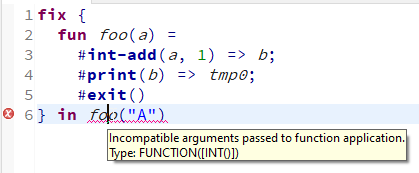
\includegraphics{img/tim_stx_inference.png}
  \caption{Type inference in the Statix specification for Tim. Statix is able to determine that the type of \texttt{a} is an integer based on its usage, and rejects the function call with the wrong argument type.}
  \label{fig:tim_statix_inference}
\end{figure}

There are several drawbacks to the Statix specification that prevent it from becoming a complete static specification for Tim. These drawbacks are also the reason why the language definition for Tim, despite the existence of a complete Statix specification, only formally specifies the name binding rules. In particular, these constraints are the following:\\

\noindent \textbf{Type signatures of primitives must be defined inside the Statix specification.} In order to properly infer types, the Statix specification must know the type signature of each primitive. Since there is no syntax to declare these signatures, they must be directly hardcoded in the specification. As a result, only a select handful of default primitives are supported by the Statix specification.\\

\noindent \textbf{The type system used is (too) simplistic}. In order to avoid specifying a complete type system for Tim, the types used in the Statix specification are very simplistic and have no concept of subtyping. New types introduced by primitives (e.g. records, arrays) are opaque and do not consider their contents. As a result, operations like \texttt{\#record-read} cannot check whether the field exists within the record. An example of this can be seen in \cref{fig:tim_statix_limitations} (top).\\

\noindent \textbf{Type inference cannot handle polymorphic functions.} The constraint solver used by Statix will unify constraints on a first-come, first-serve basis. Once a variable has been unified, any other constraints it participates in will be evaluated as equality constraints. As a result of this, a polymorphic function will unify its arguments with the first function invocation, and assume this to be the function signature. The bottom snippet in \cref{fig:tim_statix_limitations} shows this restriction. The type of \texttt{a} cannot be inferred from the body of \texttt{id}, so it is inferred from the first call (with an argument of type \texttt{INT}). The second call is then rejected, even though it would work properly at runtime.

\begin{figure}
  \begin{tim}
#record-new("foo", 1) => a;
#record-read(a, "Foo") => foo;
#print(foo) => tmp0;
#exit()
  \end{tim}
  \begin{tim}
fix {
  fun id(x, c) = c(x) // polymorphic fn(T, fn(T)) for all T
  
  fun c0() = id(1, c1) // OK, types `x` as INT()
  fun c1(_) = id("A", c2) // errors, STRING() != INT()
  fun c2(_) = #exit()
} in c0()
  \end{tim}
  \caption{Two examples of limitations within the Statix specification for Tim. In the above example, no errors are raised even though the \texttt{"Foo"} field does not exist in \texttt{a}. In the bottom example, an error is raised because the type system used in the Statix specification is unable to represent polymorphic functions.}
  \label{fig:tim_statix_limitations}
\end{figure}

\section{The Tim interpreter}
\label{sec:tim_interpreter}
In order to run Tim programs, the Spoofax implementation of Tim ships with an interpreter for the language written in Stratego. This interpreter was written as a base implementation of Tim and focuses on a correct language implementation over performance. As a result, its main purpose is the ability to run Tim programs from \textit{within} the Spoofax language workbench, such as during language development and as part of language test suites.\\

Stratego was chosen as an implementation language because it has direct integrations with most other meta-languages within the Spoofax language workbench. This allows it to be invoked from other parts of the language workbench and allows users to easily extend the language with new primitives by invoking the appropriate Stratego strategies. Since Tim reference implementation itself is also a Spoofax project, the Tim interpreter is also able to take advantage of the static type checking available in Stratego 2\footnote{Stratego 2 is a partial rewrite of the Stratego language and introduces incremental compilation and gradual typing, among other things. At the time of writing, Stratego 2 is still in development and there have yet to be any publications.}. The Tim interpreter directly implements the dynamic semantics described in \cref{sec:tim_runtime_semantics}. As such, we will refrain from discussing the entire implementation in this thesis\footnote{If the reader is interested, the code for the Tim interpreter is available online at \url{https://github.com/metaborg/spoofax-pie/blob/develop/lwb/metalang/tim_runtime/tim_runtime.spoofax2/trans}}.\\

One aspect we will briefly discuss is how the Tim interpreter performs tail calls. Neither Stratego, nor Java (to which Stratego compiles), have native support for tail calls. Since Tim is a \ac{CPS}-based language, it is imperative that it supports proper tail calls. A lack of tail call support would mean that any non-trivial Tim program will eventually run out of stack space. Tim implements tail calls very similar to the iterative approach used in its dynamic specification. Evaluating any expression will yield a continuation term, which indicates where to continue. These terms are evaluated in a \texttt{while} strategy until the program reaches termination. One particularity is that the \texttt{while} strategy from the Stratego standard library, as seen in \cref{fig:tim_interpreter_cps}, uses recursion to perform iteration. As a result, the \texttt{interpret-naive} strategy is not tail calling despite appearing to be. A custom native strategy\footnote{A Stratego strategy implemented directly in Java.} is needed to actually achieve proper tail calls.

\begin{figure}
  \begin{stratego*}{firstline=3,firstnumber=1}
module foo

strategies
  // while implemented in native code
  external native-while(c, s|)

rules
  // the while from the Stratego standard library
  while(c, s) = try(c; s; while(c, s))

  // not tail calling, since while is recursive
  interpret-naive = while(not(?Exit()); eval-expr)

  // tail calling, uses native while
  interpret-fixed = native-while(not(?Exit()); eval-expr)
  \end{stratego*}
  \caption{The \texttt{while} strategy from the Stratego standard library is implemented recursively. As a result, \texttt{interpret-naive} is not tail calling even though it appears to be.}
  \label{fig:tim_interpreter_cps}
\end{figure}

\section{Future improvements}
\label{sec:tim_future}
Let us conclude our dive into Tim by briefly discussing future improvements to the language and runtime. 

\todo[inline]{is this supposed to be in the future work chapter instead? or both?}

informal list: \todo{formalize}
\begin{itemize}
  \item Type system + better statix spec
  \item Module system
  \item Compiler/performant runtime
\end{itemize}

% - Tim grammar
% - Interpreter
% - Origins in green book
% - Primitives
% - Tim typing rules?
% - Module/type system?